% Options for packages loaded elsewhere
\PassOptionsToPackage{unicode}{hyperref}
\PassOptionsToPackage{hyphens}{url}
%
\documentclass[
]{article}
\usepackage{lmodern}
\usepackage{amsmath}
\usepackage{ifxetex,ifluatex}
\ifnum 0\ifxetex 1\fi\ifluatex 1\fi=0 % if pdftex
  \usepackage[T1]{fontenc}
  \usepackage[utf8]{inputenc}
  \usepackage{textcomp} % provide euro and other symbols
  \usepackage{amssymb}
\else % if luatex or xetex
  \usepackage{unicode-math}
  \defaultfontfeatures{Scale=MatchLowercase}
  \defaultfontfeatures[\rmfamily]{Ligatures=TeX,Scale=1}
\fi
% Use upquote if available, for straight quotes in verbatim environments
\IfFileExists{upquote.sty}{\usepackage{upquote}}{}
\IfFileExists{microtype.sty}{% use microtype if available
  \usepackage[]{microtype}
  \UseMicrotypeSet[protrusion]{basicmath} % disable protrusion for tt fonts
}{}
\makeatletter
\@ifundefined{KOMAClassName}{% if non-KOMA class
  \IfFileExists{parskip.sty}{%
    \usepackage{parskip}
  }{% else
    \setlength{\parindent}{0pt}
    \setlength{\parskip}{6pt plus 2pt minus 1pt}}
}{% if KOMA class
  \KOMAoptions{parskip=half}}
\makeatother
\usepackage{xcolor}
\IfFileExists{xurl.sty}{\usepackage{xurl}}{} % add URL line breaks if available
\IfFileExists{bookmark.sty}{\usepackage{bookmark}}{\usepackage{hyperref}}
\hypersetup{
  pdftitle={2},
  pdfauthor={Siming Yan},
  hidelinks,
  pdfcreator={LaTeX via pandoc}}
\urlstyle{same} % disable monospaced font for URLs
\usepackage[margin=1in]{geometry}
\usepackage{color}
\usepackage{fancyvrb}
\newcommand{\VerbBar}{|}
\newcommand{\VERB}{\Verb[commandchars=\\\{\}]}
\DefineVerbatimEnvironment{Highlighting}{Verbatim}{commandchars=\\\{\}}
% Add ',fontsize=\small' for more characters per line
\usepackage{framed}
\definecolor{shadecolor}{RGB}{248,248,248}
\newenvironment{Shaded}{\begin{snugshade}}{\end{snugshade}}
\newcommand{\AlertTok}[1]{\textcolor[rgb]{0.94,0.16,0.16}{#1}}
\newcommand{\AnnotationTok}[1]{\textcolor[rgb]{0.56,0.35,0.01}{\textbf{\textit{#1}}}}
\newcommand{\AttributeTok}[1]{\textcolor[rgb]{0.77,0.63,0.00}{#1}}
\newcommand{\BaseNTok}[1]{\textcolor[rgb]{0.00,0.00,0.81}{#1}}
\newcommand{\BuiltInTok}[1]{#1}
\newcommand{\CharTok}[1]{\textcolor[rgb]{0.31,0.60,0.02}{#1}}
\newcommand{\CommentTok}[1]{\textcolor[rgb]{0.56,0.35,0.01}{\textit{#1}}}
\newcommand{\CommentVarTok}[1]{\textcolor[rgb]{0.56,0.35,0.01}{\textbf{\textit{#1}}}}
\newcommand{\ConstantTok}[1]{\textcolor[rgb]{0.00,0.00,0.00}{#1}}
\newcommand{\ControlFlowTok}[1]{\textcolor[rgb]{0.13,0.29,0.53}{\textbf{#1}}}
\newcommand{\DataTypeTok}[1]{\textcolor[rgb]{0.13,0.29,0.53}{#1}}
\newcommand{\DecValTok}[1]{\textcolor[rgb]{0.00,0.00,0.81}{#1}}
\newcommand{\DocumentationTok}[1]{\textcolor[rgb]{0.56,0.35,0.01}{\textbf{\textit{#1}}}}
\newcommand{\ErrorTok}[1]{\textcolor[rgb]{0.64,0.00,0.00}{\textbf{#1}}}
\newcommand{\ExtensionTok}[1]{#1}
\newcommand{\FloatTok}[1]{\textcolor[rgb]{0.00,0.00,0.81}{#1}}
\newcommand{\FunctionTok}[1]{\textcolor[rgb]{0.00,0.00,0.00}{#1}}
\newcommand{\ImportTok}[1]{#1}
\newcommand{\InformationTok}[1]{\textcolor[rgb]{0.56,0.35,0.01}{\textbf{\textit{#1}}}}
\newcommand{\KeywordTok}[1]{\textcolor[rgb]{0.13,0.29,0.53}{\textbf{#1}}}
\newcommand{\NormalTok}[1]{#1}
\newcommand{\OperatorTok}[1]{\textcolor[rgb]{0.81,0.36,0.00}{\textbf{#1}}}
\newcommand{\OtherTok}[1]{\textcolor[rgb]{0.56,0.35,0.01}{#1}}
\newcommand{\PreprocessorTok}[1]{\textcolor[rgb]{0.56,0.35,0.01}{\textit{#1}}}
\newcommand{\RegionMarkerTok}[1]{#1}
\newcommand{\SpecialCharTok}[1]{\textcolor[rgb]{0.00,0.00,0.00}{#1}}
\newcommand{\SpecialStringTok}[1]{\textcolor[rgb]{0.31,0.60,0.02}{#1}}
\newcommand{\StringTok}[1]{\textcolor[rgb]{0.31,0.60,0.02}{#1}}
\newcommand{\VariableTok}[1]{\textcolor[rgb]{0.00,0.00,0.00}{#1}}
\newcommand{\VerbatimStringTok}[1]{\textcolor[rgb]{0.31,0.60,0.02}{#1}}
\newcommand{\WarningTok}[1]{\textcolor[rgb]{0.56,0.35,0.01}{\textbf{\textit{#1}}}}
\usepackage{longtable,booktabs}
\usepackage{calc} % for calculating minipage widths
% Correct order of tables after \paragraph or \subparagraph
\usepackage{etoolbox}
\makeatletter
\patchcmd\longtable{\par}{\if@noskipsec\mbox{}\fi\par}{}{}
\makeatother
% Allow footnotes in longtable head/foot
\IfFileExists{footnotehyper.sty}{\usepackage{footnotehyper}}{\usepackage{footnote}}
\makesavenoteenv{longtable}
\usepackage{graphicx}
\makeatletter
\def\maxwidth{\ifdim\Gin@nat@width>\linewidth\linewidth\else\Gin@nat@width\fi}
\def\maxheight{\ifdim\Gin@nat@height>\textheight\textheight\else\Gin@nat@height\fi}
\makeatother
% Scale images if necessary, so that they will not overflow the page
% margins by default, and it is still possible to overwrite the defaults
% using explicit options in \includegraphics[width, height, ...]{}
\setkeys{Gin}{width=\maxwidth,height=\maxheight,keepaspectratio}
% Set default figure placement to htbp
\makeatletter
\def\fps@figure{htbp}
\makeatother
\setlength{\emergencystretch}{3em} % prevent overfull lines
\providecommand{\tightlist}{%
  \setlength{\itemsep}{0pt}\setlength{\parskip}{0pt}}
\setcounter{secnumdepth}{-\maxdimen} % remove section numbering
\usepackage{booktabs}
\usepackage{longtable}
\usepackage{array}
\usepackage{multirow}
\usepackage{wrapfig}
\usepackage{float}
\usepackage{colortbl}
\usepackage{pdflscape}
\usepackage{tabu}
\usepackage{threeparttable}
\usepackage{threeparttablex}
\usepackage[normalem]{ulem}
\usepackage{makecell}
\usepackage{xcolor}
\ifluatex
  \usepackage{selnolig}  % disable illegal ligatures
\fi

\title{2}
\author{Siming Yan}
\date{01 February, 2021}

\begin{document}
\maketitle

\hypertarget{data-preview}{%
\subsection{Data preview}\label{data-preview}}

\hypertarget{ux4e00-ux8bf7ux95eeux8fd9ux4e09ux4e2aux4ebaux7684ux773cux775bux662fux4ec0ux4e48ux989cux8272ux7684ux8981ux6c42ux7ed9ux51faux63a8ux7406ux8fc7ux7a0b}{%
\subsection{一、
请问这三个人的眼睛是什么颜色的,要求给出推理过程。}\label{ux4e00-ux8bf7ux95eeux8fd9ux4e09ux4e2aux4ebaux7684ux773cux775bux662fux4ec0ux4e48ux989cux8272ux7684ux8981ux6c42ux7ed9ux51faux63a8ux7406ux8fc7ux7a0b}}

{\emph{Ans:}第二天自杀的两位是绿色(G),第三天自杀的是黄色(Y)。}

{\emph{Ans:}推理过程:假设三个人分别叫A B
C,第一天三个人都没自杀,说明他们三个人都不能确定自己的身份,
鉴于必须至少有一个绿色(G),那么组合如下:}

\begin{longtable}[]{@{}lll@{}}
\toprule
A & B & C\tabularnewline
\midrule
\endhead
Y & G & G\tabularnewline
G & G & Y\tabularnewline
G & Y & G\tabularnewline
G & G & G\tabularnewline
\bottomrule
\end{longtable}

\emph{Ans:}第一天某两个人眼中所见为一黄一绿(设:A
B),剩余一人所见为两绿(设:C)。不确定绿色有2人还是3人,所以他们不敢自杀。第二天发现没有人死以后,他们推断出了这一种组合方式。因此A
B明白:自己就是绿色的!因为如果自己是黄色,那对方应该第一天就发现另外两人是黄色而自杀。所以第二日AB自杀,自报绿色。第三天C自杀,因为AB敢于自杀,推断出AB眼中所见一直是一黄一绿。

\begin{center}\rule{0.5\linewidth}{0.5pt}\end{center}

\hypertarget{ux4e8c-ux8bf7ux4e8cux9009ux4e00ux4f5cux7b54}{%
\subsection{二、
请二选一作答}\label{ux4e8c-ux8bf7ux4e8cux9009ux4e00ux4f5cux7b54}}

1、 如果不受限制,你希望做什么样的游戏,为什么值得做这个游戏?

{\emph{Ans:}做更好的VR游戏,身临其境的开放式世界,如GTA5,cyberpunk2077,给人类一个新世界!像黑镜中的世界一样,人类或许可以因此获得永生的机会,又或许就像elon
mask 一样,开辟``火星'',新的家园。}

\begin{center}\rule{0.5\linewidth}{0.5pt}\end{center}

\hypertarget{ux4e09-ux8bf7ux6309ux7167ux9644ux4ef6excelux4e2dux7684ux6570ux636eux5206ux6790ux8bf7ux89c1ux9644ux4ef6abcux4e09ux4e2aux5f53ux4e2dux6309ux7167ux6bdbux6536ux5165ux6210ux672cux5229ux6da6ux7387ux5217ux964dux5e8fux6392ux5217ux6211ux4eecux91c7ux7528ux54eaux79cdux6295ux5165ux65b9ux6848ux6027ux4ef7ux6bd4ux6700ux9ad8-ux7ed9ux51faux7406ux7531ux5f00ux653eux5f0fux5fc5ux7b54ux9898}{%
\subsection{三、
请按照附件excel中的数据分析(请见附件)ABC三个当中(按照毛收入/成本(利润率)列,降序排列)我们采用哪种投入方案,性价比最高?
给出理由。(开放式,必答题)}\label{ux4e09-ux8bf7ux6309ux7167ux9644ux4ef6excelux4e2dux7684ux6570ux636eux5206ux6790ux8bf7ux89c1ux9644ux4ef6abcux4e09ux4e2aux5f53ux4e2dux6309ux7167ux6bdbux6536ux5165ux6210ux672cux5229ux6da6ux7387ux5217ux964dux5e8fux6392ux5217ux6211ux4eecux91c7ux7528ux54eaux79cdux6295ux5165ux65b9ux6848ux6027ux4ef7ux6bd4ux6700ux9ad8-ux7ed9ux51faux7406ux7531ux5f00ux653eux5f0fux5fc5ux7b54ux9898}}

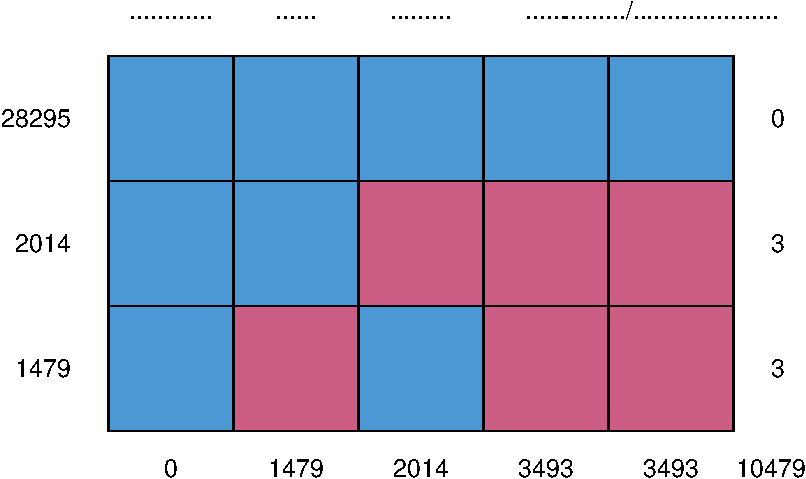
\includegraphics{yansiming_dataScience_files/figure-latex/unnamed-chunk-2-1.pdf}

\begin{verbatim}
      产品代码 成本 毛收入 利润 毛收入/成本(利润率)      
28295        1    1      1    1                     1     0
2014         1    1      0    0                     0     3
1479         1    0      1    0                     0     3
             0 1479   2014 3493                  3493 10479
\end{verbatim}

\hypertarget{sort-data-in-decreasing-order.}{%
\paragraph{sort data in decreasing
order.}\label{sort-data-in-decreasing-order.}}

\begin{Shaded}
\begin{Highlighting}[]
\NormalTok{data }\OtherTok{=}\NormalTok{ data[}\FunctionTok{order}\NormalTok{(data}\SpecialCharTok{$}\StringTok{\textasciigrave{}}\AttributeTok{毛收入/成本(利润率)}\StringTok{\textasciigrave{}}\NormalTok{, }\AttributeTok{decreasing =}\NormalTok{ T), ]}
\end{Highlighting}
\end{Shaded}

\hypertarget{remove-nas-in-ux6bdbux6536ux5165ux6210ux672cux5229ux6da6ux7387}{%
\paragraph{\texorpdfstring{remove NAs in
\texttt{毛收入/成本(利润率)}}{remove NAs in 毛收入/成本(利润率)}}\label{remove-nas-in-ux6bdbux6536ux5165ux6210ux672cux5229ux6da6ux7387}}

\begin{Shaded}
\begin{Highlighting}[]
\NormalTok{data\_nna }\OtherTok{=}\NormalTok{ data[}\SpecialCharTok{{-}}\FunctionTok{which}\NormalTok{(}\FunctionTok{is.na}\NormalTok{(data}\SpecialCharTok{$}\StringTok{\textasciigrave{}}\AttributeTok{毛收入/成本(利润率)}\StringTok{\textasciigrave{}}\NormalTok{) }\SpecialCharTok{==}\NormalTok{ T), ]}
\end{Highlighting}
\end{Shaded}

\begin{Shaded}
\begin{Highlighting}[]
\NormalTok{data }\OtherTok{=}\NormalTok{ data\_nna}
\NormalTok{data\_nna }\OtherTok{=}\NormalTok{ data\_nna[}\FunctionTok{order}\NormalTok{(data\_nna}\SpecialCharTok{$}\NormalTok{利润, }\AttributeTok{decreasing =}\NormalTok{ T), ]}
\end{Highlighting}
\end{Shaded}

\hypertarget{solve}{%
\paragraph{solve}\label{solve}}

\begin{Shaded}
\begin{Highlighting}[]
\NormalTok{total\_sale }\OtherTok{=} \FunctionTok{sum}\NormalTok{(data\_nna}\SpecialCharTok{$}\NormalTok{利润)}
\FunctionTok{c}\NormalTok{(total\_sale }\SpecialCharTok{*} \FloatTok{0.7}\NormalTok{, total\_sale }\SpecialCharTok{*} \FloatTok{0.8}\NormalTok{, total\_sale }\SpecialCharTok{*} \FloatTok{0.925}\NormalTok{)}
\end{Highlighting}
\end{Shaded}

\begin{verbatim}
[1] 11286160 12898468 14913854
\end{verbatim}

\begin{Shaded}
\begin{Highlighting}[]
\NormalTok{out\_a }\OtherTok{=} \ControlFlowTok{for}\NormalTok{ (i }\ControlFlowTok{in} \DecValTok{1}\SpecialCharTok{:}\FunctionTok{dim}\NormalTok{(data\_nna)[}\DecValTok{1}\NormalTok{]) \{}
    \ControlFlowTok{if}\NormalTok{ (}\FunctionTok{sum}\NormalTok{(data\_nna[}\DecValTok{1}\SpecialCharTok{:}\NormalTok{i, ]}\SpecialCharTok{$}\NormalTok{利润) }\SpecialCharTok{\textgreater{}=}\NormalTok{ total\_sale }\SpecialCharTok{*} \FloatTok{0.7}\NormalTok{) \{}
        \FunctionTok{print}\NormalTok{(i)}
        \ControlFlowTok{break}
\NormalTok{    \}}
\NormalTok{\}}
\end{Highlighting}
\end{Shaded}

\begin{verbatim}
[1] 197
\end{verbatim}

\begin{Shaded}
\begin{Highlighting}[]
\NormalTok{out\_a2 }\OtherTok{=} \FunctionTok{sum}\NormalTok{(data\_nna[}\DecValTok{1}\SpecialCharTok{:}\DecValTok{197}\NormalTok{, ]}\SpecialCharTok{$}\NormalTok{利润)}
\NormalTok{out\_a3 }\OtherTok{=} \FunctionTok{sum}\NormalTok{(data\_nna[}\DecValTok{1}\SpecialCharTok{:}\DecValTok{197}\NormalTok{, ]}\SpecialCharTok{$}\NormalTok{成本)}\SpecialCharTok{/}\FunctionTok{sum}\NormalTok{(data\_nna}\SpecialCharTok{$}\NormalTok{成本)}
\NormalTok{out\_a4 }\OtherTok{=} \FunctionTok{sum}\NormalTok{(data\_nna[}\DecValTok{1}\SpecialCharTok{:}\DecValTok{197}\NormalTok{, ]}\SpecialCharTok{$}\NormalTok{毛收入)}\SpecialCharTok{/}\FunctionTok{sum}\NormalTok{(data\_nna}\SpecialCharTok{$}\NormalTok{成本)}
\end{Highlighting}
\end{Shaded}

{\emph{Ans:} A方案产品一共197个, 利润总额11289488, 成本占比0.55697,
总体利润率5.27993}

\begin{Shaded}
\begin{Highlighting}[]
\NormalTok{out\_b }\OtherTok{=} \ControlFlowTok{for}\NormalTok{ (i }\ControlFlowTok{in} \DecValTok{1}\SpecialCharTok{:}\FunctionTok{dim}\NormalTok{(data\_nna)[}\DecValTok{1}\NormalTok{]) \{}
    \ControlFlowTok{if}\NormalTok{ (}\FunctionTok{sum}\NormalTok{(data\_nna[}\DecValTok{1}\SpecialCharTok{:}\NormalTok{i, ]}\SpecialCharTok{$}\NormalTok{利润) }\SpecialCharTok{\textgreater{}=}\NormalTok{ total\_sale }\SpecialCharTok{*} \FloatTok{0.8}\NormalTok{) \{}
        \FunctionTok{print}\NormalTok{(i)}
        \ControlFlowTok{break}
\NormalTok{    \}}
\NormalTok{\}}
\end{Highlighting}
\end{Shaded}

\begin{verbatim}
[1] 381
\end{verbatim}

\begin{Shaded}
\begin{Highlighting}[]
\NormalTok{out\_b2 }\OtherTok{=} \FunctionTok{sum}\NormalTok{(data\_nna[}\DecValTok{1}\SpecialCharTok{:}\DecValTok{381}\NormalTok{, ]}\SpecialCharTok{$}\NormalTok{利润)}
\NormalTok{out\_b3 }\OtherTok{=} \FunctionTok{sum}\NormalTok{(data\_nna[}\DecValTok{1}\SpecialCharTok{:}\DecValTok{381}\NormalTok{, ]}\SpecialCharTok{$}\NormalTok{成本)}\SpecialCharTok{/}\FunctionTok{sum}\NormalTok{(data\_nna}\SpecialCharTok{$}\NormalTok{成本)}
\NormalTok{out\_b4 }\OtherTok{=} \FunctionTok{sum}\NormalTok{(data\_nna[}\DecValTok{1}\SpecialCharTok{:}\DecValTok{381}\NormalTok{, ]}\SpecialCharTok{$}\NormalTok{毛收入)}\SpecialCharTok{/}\FunctionTok{sum}\NormalTok{(data\_nna}\SpecialCharTok{$}\NormalTok{成本)}
\end{Highlighting}
\end{Shaded}

{\emph{Ans:} B方案产品一共381个, 利润总额12902319,
成本占比0.67366,总体利润率6.07134}

\begin{Shaded}
\begin{Highlighting}[]
\ControlFlowTok{for}\NormalTok{ (i }\ControlFlowTok{in} \DecValTok{1}\SpecialCharTok{:}\FunctionTok{dim}\NormalTok{(data\_nna)[}\DecValTok{1}\NormalTok{]) \{}
    \ControlFlowTok{if}\NormalTok{ (}\FunctionTok{sum}\NormalTok{(data\_nna[}\DecValTok{1}\SpecialCharTok{:}\NormalTok{i, ]}\SpecialCharTok{$}\NormalTok{利润) }\SpecialCharTok{\textgreater{}=}\NormalTok{ total\_sale }\SpecialCharTok{*} \FloatTok{0.925}\NormalTok{) \{}
        \FunctionTok{print}\NormalTok{(i)}
        \ControlFlowTok{break}
\NormalTok{    \}}
\NormalTok{\}}
\end{Highlighting}
\end{Shaded}

\begin{verbatim}
[1] 1288
\end{verbatim}

\begin{Shaded}
\begin{Highlighting}[]
\NormalTok{out\_c2 }\OtherTok{=} \FunctionTok{sum}\NormalTok{(data\_nna[}\DecValTok{1}\SpecialCharTok{:}\DecValTok{1288}\NormalTok{, ]}\SpecialCharTok{$}\NormalTok{利润)}
\NormalTok{out\_c3 }\OtherTok{=} \FunctionTok{sum}\NormalTok{(data\_nna[}\DecValTok{1}\SpecialCharTok{:}\DecValTok{1288}\NormalTok{, ]}\SpecialCharTok{$}\NormalTok{成本)}\SpecialCharTok{/}\FunctionTok{sum}\NormalTok{(data\_nna}\SpecialCharTok{$}\NormalTok{成本)}
\NormalTok{out\_c4 }\OtherTok{=} \FunctionTok{sum}\NormalTok{(data\_nna[}\DecValTok{1}\SpecialCharTok{:}\DecValTok{1288}\NormalTok{, ]}\SpecialCharTok{$}\NormalTok{毛收入)}\SpecialCharTok{/}\FunctionTok{sum}\NormalTok{(data\_nna}\SpecialCharTok{$}\NormalTok{成本)}
\end{Highlighting}
\end{Shaded}

{\emph{Ans:}C方案产品一共1288个, 利润总额14914188,
成本占比0.85155,总体利润率7.0909}

{\emph{Ans:} 选择方案C, 总体利润率最高}

\begin{center}\rule{0.5\linewidth}{0.5pt}\end{center}

\hypertarget{ux56db-ux67d0ux7535ux5546ux5e73ux53f0ux4e3bux8981ux9762ux5411ux7684ux7528ux6237ux7fa4ux4e3aux5973ux6027ux767dux9886ux6700ux8fd17ux5929ux9500ux552eux91d1ux989dux5982ux4e0bux8868}{%
\subsection{四、
某电商平台主要面向的用户群为女性白领,最近7天销售金额如下表}\label{ux56db-ux67d0ux7535ux5546ux5e73ux53f0ux4e3bux8981ux9762ux5411ux7684ux7528ux6237ux7fa4ux4e3aux5973ux6027ux767dux9886ux6700ux8fd17ux5929ux9500ux552eux91d1ux989dux5982ux4e0bux8868}}

{\emph{Ans:}
工作日销售量更多。原因有:1、可能产品广告投放在工作用的app或者网页中,或者通勤路线上。2、类似于外卖,下午茶,咖啡,功能饮料,对工作有所帮助或者能增添工作时期虚荣心的产品。3、会议设备等工作相关的必需品租赁。改进计划:增添其他渠道的广告投放,坐在家里也要看到我们的产品;通过社交软件进行宣传,提升虚拟价值,让白领在家也有所炫耀;推出风险对冲产品,上班喝咖啡,周末在家买花茶,燕窝护肤缓解疲劳
etc。}

\end{document}
